\documentclass[12pt]{article} % Define document class

%% Main package imports with descriptions
\usepackage{graphicx, amsmath}
% Usepackage{{for images}{for referencing equations with numbers}}

\graphicspath{{./img/}} % graphicx: define path for images

% Hyperlinks in PDF:
\usepackage{hyperref, color}
\definecolor{linkcolor}{rgb}{0,0,0.4}
\hypersetup{
		breaklinks=true,
		colorlinks=true,
		linkcolor=linkcolor,
		urlcolor=linkcolor,
		citecolor=black,
		filecolor=black,
		%filecolor=blue,
		pdfmenubar=true,
		pdftoolbar=true,
		bookmarksdepth=3   % Uncomment (and tweak) for PDF bookmarks with more levels than the TOC
	    }


%%%%%%%%%%%%%%%%%%%%%%%%%%%%%%%%%%%%%%%%%%%%%%%%%%%%%%%%%%%%%%%%%%%%%%%%%%%%%%
\begin{document}
\title{Project 4: Financial Engineering from a Statistical Physics Approach}
\author{Michael Saybolt}
\date{5/7/2017}
\maketitle
\pagebreak

\tableofcontents

\begin{abstract} % Present tense
This project explores the generation and simulation of an economic system. Financial transactions among agents are simulated using Monte Carlo methods. The resulting distribution of wealth is then studied. Various parameters can be tuned to create a system that accurately models real wealth distributions from various countries.
\end{abstract}

\section{Introduction} % Rest of paper, past tense
The end goal is to analyze the distribution of wealth as a function of agents'
money/income, \textit{m}. The result should follow a Pareto distribution
\cite{Pareto}. In addition, the model was made more realistic by following the
work of
\href{{http://www.sciencedirect.com/science/article/pii/S0378437104004327}}{Patriarca
and collaborators}, adding a quantity $\lambda$ responsible for making the
agents save a certain fraction of their money during a transaction
\cite{Patriarca}.
Following the work of
\href{{http://www.sciencedirect.com/science/article/pii/S0378437114006967}}{Goswami
and Sen}, the agents can be further enhanced to model tendencies to interact
with other agents of similar income, as well as previous
interactions\cite{Goswami}.


\section{Technical Details}
\subsection{General Considerations}
In all levels of modeling, there are some basic considerations that may differ
slightly from the papers. In general, the distribution of money follows
\[
w_m\propto m^{-1-\alpha},
\]
with $\alpha\in [1,2]$\cite{Pareto}.

A certain number of agents N are created for each Monte Carlo iteration, and
they are randomly selected to perform transactions. Unlike the paper, they are
each assigned some equal start money, \textit{$m_0$}, instead of a random value
from a uniform distribution. The choosing of the agents, however, is still done
using a uniform distribution. \texttt{For} some number of Monte Carlo cycles,
\texttt{for} some number of transactions, a pair of agents
(\textit{i},\textit{j}) are chosen by the uniform distribution, and exchange
money. Money is conserved, thus
\begin{equation}
  m_i+m_j=m_i'+m_j'.
  \label{eq:conserve}
\end{equation}
The random number $\epsilon$, generated from a uniform distribution, is used to
determine the fraction of money that is changed. The money of agents'
\textit{i} and \textit{j} become
\begin{equation*}
m_i' = \epsilon(m_i+m_j),
\end{equation*}
leading to
\begin{equation*}
m_j'= (1-\epsilon)(m_i+m_j).
\end{equation*}
No agents can go into debt (only finitely smaller transactions), and due to the
conservation law, the system relaxes towards a Gibbs distribution.

\subsection{Parameter Choice}
Parameters are chosen initially such that when the system reaches its
termmination condition, there are not 'holes' in the data set. Without
sufficient interactions, and more importantly enough Monte Carlo cycles to even
out the dataset, there will be parts of the distribution of wealth with no
agents in that section. Taking the log of the distribution of wealth will look
uneven and be inaccurate as a result, when it should look relatively linear for
the most basic economic model (no money saved or other caveats to interaction).
Additionally, sufficient start money seemed to play a role (even though it
seems it shouldn't, as all floats tested can be divided or multiplied many
times themselves without significant accuracy loss), however there was not
enough CPU time to verify this trend.

\subsection{Termination Conditions}
The termination condition is met when the system has reached some sort of equilibrium.
This can be guessed by looking at the data and seeing when it quits changing
much with additional transactions, or for a more quantatative approach, the variance
amongst the agents can be observed as the transactions go on, which will
stabilize when the system reaches equilibrium.
\newcommand{\scaleVar}{0.5}
\begin{figure}
	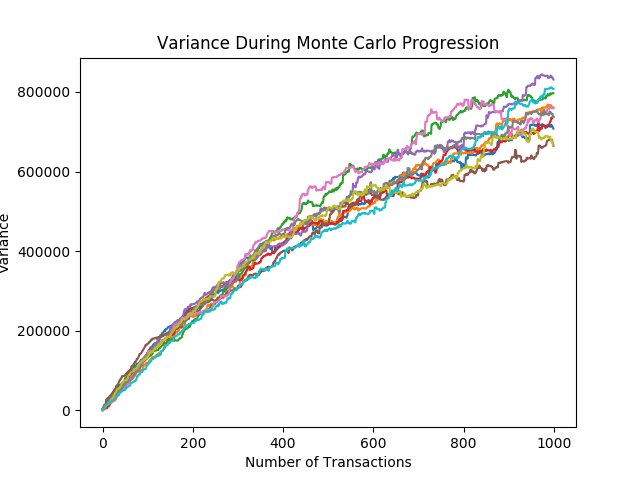
\includegraphics[scale=\scaleVar]{variancenotconverged.png}
	%\centering
	\caption{Variance of 10 Monte Carlo cycles with
	\texttt{num\_transactions}=$10^3$}
	\label{fig:variancenotconverged}
\end{figure}
\begin{figure}
	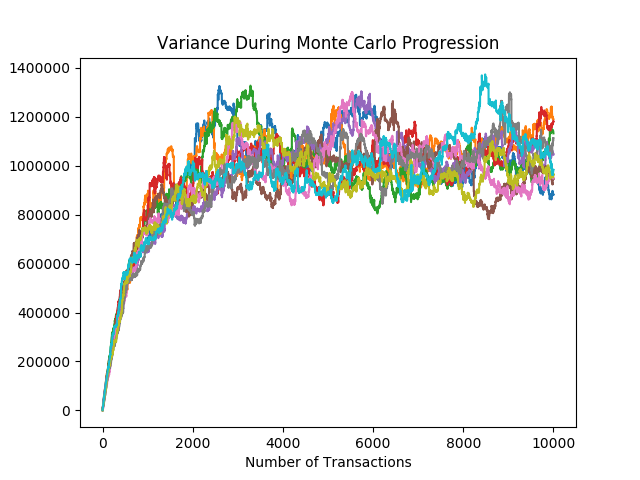
\includegraphics[scale=\scaleVar]{varianceconverged.png}
	\caption{Variance of 10 Monte Carlo cycles with
	\texttt{num\_transactions}=$10^4$
	\label{fig:varianceconverged}
\end{figure}
\begin{figure}
	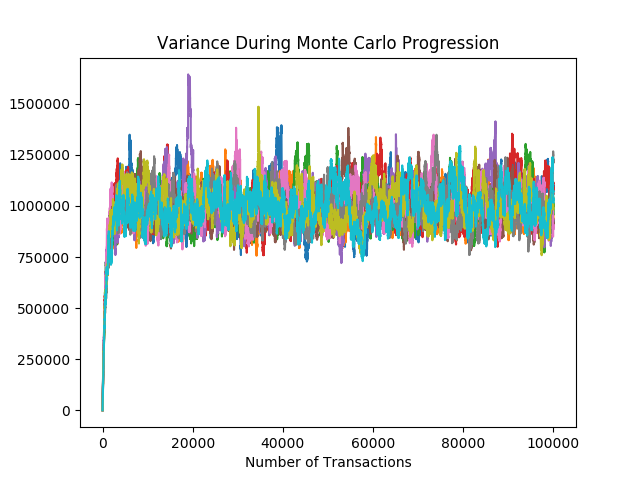
\includegraphics[scale=\scaleVar]{variancefullyconverged.png}	
	\caption{Variance of 10 Monte Carlo cycles with
	\texttt{num\_transactions}=$10^5$
	\label{fig:variancefullyconverged}
\end{figure}
Figures \ref{fig:variancenotconverged}, \ref{fig:varianceconverged}, and
\ref{fig:variancefullyconverged} show the variance against number of
transactions and 10 Monte Carlo cycles for clarity. Choosing
\texttt{num\_transactions} to ensure the system is at equilibrium is no longer
a guessing game. This tends to be very predictable, and unless the number of
agents \texttt{N} is changed, the system's convergence to equilibrium is easily
predicted within an order of magnitude.

\section{Big Data Challenges}
\subsection{Dealing with Large Sets of Data}
Unlike previous projects, Monte Carlo simulations involve a lot of CPU time to
generate a sufficient pool of pseudo randomly generated data. While some
general trends can be observed with less iterations for debugging, to truly
check the details, sufficient numbers of experiments must be done.

This prompted the need for modularizing the code, building a libray for
commonly used functions, adding load and store functions, as well as a
separate program \texttt{quikplot} to just plot data. Running through all that computation just
to plot something and then discard it after making changes to the code is
incredibly wasteful and inefficient, so after the cycles complete, it
optionally writes to a file and/or plots, using functions contained in a shared
financial library. This way, a separate plotting function can load the files
into variables and call the exact same plotting function to recreate and
display that environment.

\subsection{Computation of Large Sets of Data}
\subsubsection{Parallelization Attempt}
When dealing with such a CPU intensive task, parallelization immediately comes
to mind. Unfortunately parallelizing the Monte Carlo cycles did not seem
trivial, at least in the stage of the code that was first attempted to be
parallelized. This seemed strange, as individual cycles do not depend on each
other unless the termination condition relies on comparing other cycles and
must index them numerically during computation.

\subsubsection{Crude but Effective Method}
Since CPU time is of essence near the end of the semester, utilizing as much of
it as possible is still a top priority. While my ~4 GHz antenna simulation
targeted desktop can kick out more flops than the engineering building's
compute servers core-per-core, the compute servers have many, many more cores.
Just dying for a parallel implementation of this code. Since parameters needed
to be varied for the extra details and caveats of the transactions, multiple
python instances can be started separately, and then data combined at the end,
programatically, but not truly 'parallel' code.

\begin{figure}
	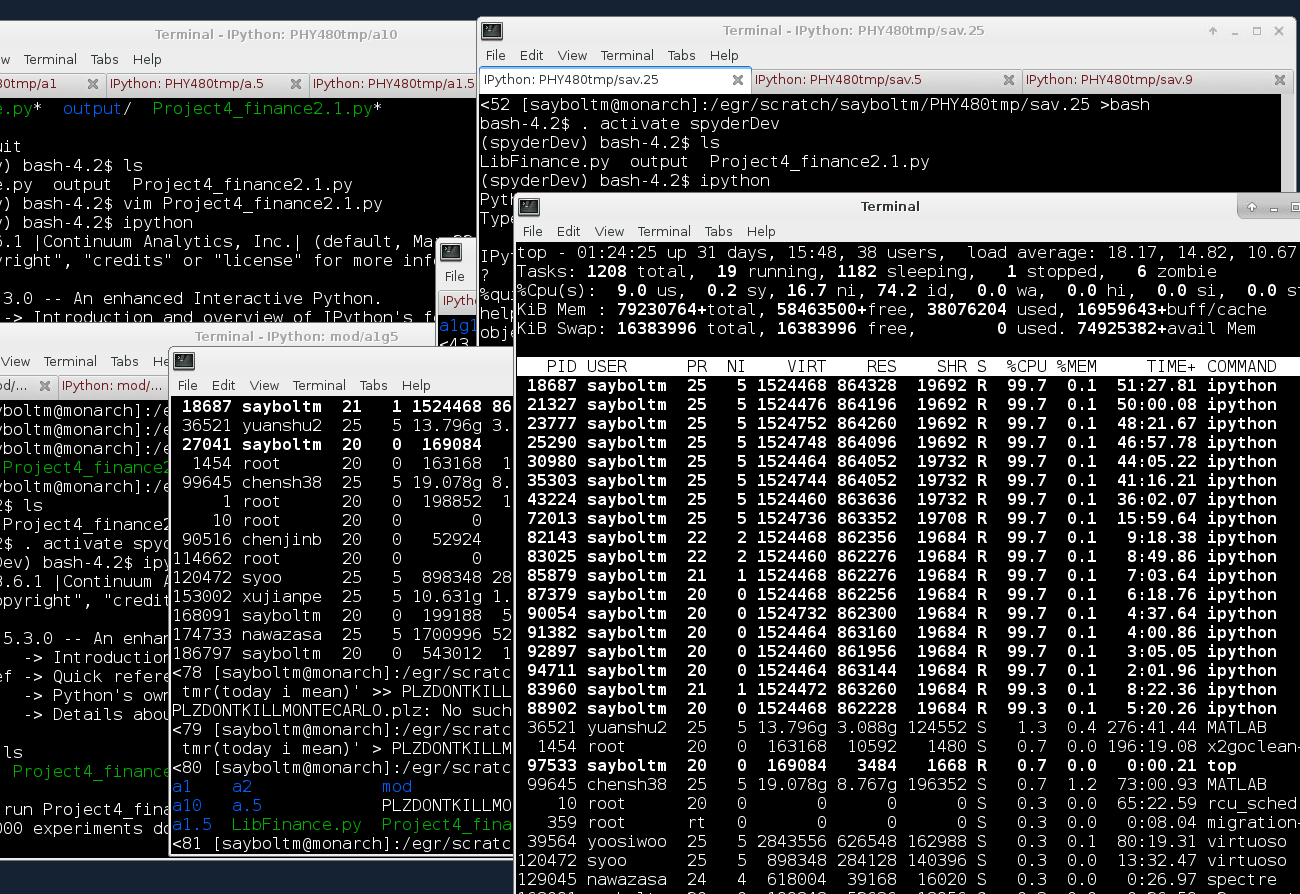
\includegraphics[scale=0.75]{LOL.PNG}
	\centering
	\caption{Taking over the engineering compute servers}
	\label{fig:computeuse}
\end{figure}

Of course care was taken to use the least loaded one, but running 30+ instances
of Python on cores half as fast was still a much faster way to acquire large
sets of reasonably accurate data!

\section{Results}
A formal discussion of the results of adjusting the model to more accurately
represent real economic principals is presented.

\subsection{Default}
The 'default' model simply follows exponential decay as mentioned in the
introduction \cite{Pareto}. Agents do not save any money, nor do they
discriminate based on wealth or previous transaction. There are many agents
with little money, and very few with a lot of money.
\newcommand{\scaleResults}{0.75}
\begin{figure}
	\includegraphics[scale=\scaleResults]{}
	\caption{Pareto distribution}
\end{figure}

Taking the log of this function results in a relatively straight line, so long
as enough interactions take place.
\begin{figure}
	\includegraphics[scale=\scaleResults]{}
	\caption{Log of the 'default' Gibbs distribution}
\end{figure}

\subsection{Savings}
To add realism or study a hypothetical economic systme, agents can save a
fraction of their money, $\lambda$, in a transaction. While equation
\eqref{eq:conserve} for conservation of money still holds, the new money of
the agents is modeled as follows
\begin{equation*}
  m_i' = \lambda m_i+\epsilon(1-\lambda)(m_i+m_j),
\end{equation*}

and

\begin{equation*}
  m_j' = \lambda m_j+(1-\epsilon)(1-\lambda)(m_i+m_j),
\end{equation*}

When agents save money, a strong 'middle class' is born. Results for saving a
quarter, half and 90\% of their money is shown.

\begin{figure}
	\includegraphics[scale=\scaleResults]{}
	\caption{Distribution of wealth for $\lambda$=0.25}
	\label{}
\end{figure}


\begin{figure}
	\includegraphics[scale=\scaleResults]{}
	\caption{Distribution of wealth for $\lambda$=0.5}
	\label{}
\end{figure}
\begin{figure}
	\includegraphics[scale=\scaleResults]{}
	\caption{Distribution of wealth for $\lambda$=0.9}
	\label{}
\end{figure}

\subsection{Similar Wealth}
Agents can also be tailored to be more likely to interact with other agents of
similar wealth, or geographic proximity, regardless of how much they save. This seems to help the lower and
mid-income agents, and if the log is taken, somewhat resembles the plots in
Goswami and Sen\cite{Goswami}.

\begin{figure}
	\includegraphics[scale=\scaleResults]{}
	\caption{Distribution of wealth for $\alpha$=0.5}
	\label{}
\end{figure}

\begin{figure}
	\includegraphics[scale=\scaleResults]{}
	\caption{Distribution of wealth for $\alpha$=1.0}
	\label{}
\end{figure}
\begin{figure}
	\includegraphics[scale=\scaleResults]{}
	\caption{Distribution of wealth for $\alpha$=1.5}
	\label{}
\end{figure}
\begin{figure}
	\includegraphics[scale=\scaleResults]{}
	\caption{Distribution of wealth for $\alpha$=2.0}
	\label{}
\end{figure}

Taking it to the max to really see the influence

\begin{figure}
	\includegraphics[scale=\scaleResults]{}
	\caption{Distribution of wealth for $\alpha$=10}
	\label{}
\end{figure}

\subsection{Adding Previous Interactions}
People may have a tendency to want to continue to do business with previous
clients, assuming it was a good transaction. Multiplying the probability of an
interaction based on similar wealth, with an additional component containing a
comparison to the maximum transactions between any agents, a confidence factor
can be added in, increasing the likelhood of a transaction occuring the more
previous transactions some agents have with each other.


\section{Conclusions and Future Work}


\begin{thebibliography}{2} % Bib must be called thebibliography
		% Bib changes to bib if doctype=book or something,
		% doctype=article makes it print references
		%The number supposedly needs to match the num refs but doesn't
		%seem so
\bibitem{Pareto}
\href{{http://www.institutcoppet.org/2012/05/08/cours-deconomie-politique-1896-de-vilfredo-pareto}}{V. Pareto, Cours d'economie politique, Lausanne, 1897}.

\bibitem{Patriarca}	
\href{{http://www.sciencedirect.com/science/article/pii/S0378437104004327}}{M. Patriarca, A. Chakraborti, K. Kaski, Physica A \textbf{340}, 334 (2004)}.

\bibitem{Goswami}
\href{{http://www.sciencedirect.com/science/article/pii/S0378437114006967}}{S. Goswami and P. Sen, Physica A \textbf{415}, 514 (2014)}.
%moar
%https://www.sharelatex.com/learn/Bibliography_management_with_bibtex?&nocdn=true
\end{thebibliography}
\end{document}
